%!TEX root = ../template.tex
%%%%%%%%%%%%%%%%%%%%%%%%%%%%%%%%%%%%%%%%%%%%%%%%%%%%%%%%%%%%%%%%%%%%
%% chapter4.tex
%% NOVA thesis document file
%%
%% Chapter with lots of dummy text
%%%%%%%%%%%%%%%%%%%%%%%%%%%%%%%%%%%%%%%%%%%%%%%%%%%%%%%%%%%%%%%%%%%%

\typeout{NT FILE chapter4.tex}%

\chapter{Related Work}
\label{cha:related_work}

As mentioned in Section 1, this work will encompass the development of
mechanisms for evaluating and managing the soundness of updates in RESTfull service contracts.
We now summarize the most significant pieces of work from the literature
that relate to the evolution of microservices and their APIs.

\section{Web API Description Languages} % (fold)
\label{sec:web_api_description_languages}

Web API development has risen dramatically in recent years;  unlike statically linked library APIs,
where developers may choose to stick with an earlier version that met their needs, with web APIs,
the provider can discontinue a specific version and capability at any moment.
This represents a heavy burden for client developers as it causes an endless struggle to keep up
with changes pushed by the web API providers; this load is exacerbated if the web API is inadequately documented.

\paragraph{}

Web API Description Languages (WADL) are domain-specific languages used to describe web service contracts in a standardized structure;
also sometimes referred to as interface description languages (IDLs).

These structured descriptions might be used to produce documentation for human programmers, that is easier to read than free-form documentation,
since all documentation generated by the same tool adheres to the same formatting norms.
Furthermore, description languages are often accurate enough to allow for the automatic generation of various software artifacts such as mock servers,
client code generation in different programming languages, load test scripts, and so on.

\paragraph{}

The OpenAPI Specification (OAS) is the most widely adopted Restful API Description Language;
it defines a standard, language-agnostic interface that allows both humans and computers to discover and
understand the capabilities of a service without access to source code, documentation, or network traffic inspection.
When properly defined, a consumer can understand and interact with the remote service with a minimal amount of implementation logic.

OpenApi allows a detailed description of the syntactic aspects of the data transferred in REST interactions, however it ignores important semantic aspects, such as the ability to relate
different parts of the same data, to relate the input against the state of the service, and to relate the output against the input.

For instance, OpenAPI does not allow developers to indicate that the type of representation conveyed in the response to a GET operation is dependent on the value of a query parameter.

\paragraph{}

The paper "HeadREST: A Specification Language for
RESTful APIs" \cite{16} proposes an alternative WADL that supports the expression of semantic aspects in data. Two ideas are embodied in the proposed description language:

\paragraph{Refinement Types} can be used to express the properties of data exchanged.
A refinement type x can be defined as:
\[ x:T -> e \]
Where x is an object of the primitive type T, and e is a predicate which returns true or false depending on whether the value conforms to the boolean expression (eg. x > 10).

\paragraph{Pre- and post-conditions} can be used to express relationships between data sent in
requests, and the data returned in responses. These conditions can be expressed as a collection of Hoare triple assertions
\[ \phi (a : t) \psi \]
Where a is REST operation type (GET, POST, PUT, or DELETE),
t is an URI template (e.g. /users/),
and φ and ψ are boolean expressions.
Formula φ, called the pre-condition, addresses the state in which the action is performed as well as the data transmitted in the request,
whereas ψ, the post-condition, addresses the state resulting from the execution of the operation together with the values transmitted in the response.

\paragraph{}

Our solution will require the use on WADL for defining compatibility relations between service contracts,
as well for the implementation of the adaptation protocol, which alters messages in accordance to an earlier contract.

The OpenAPI specification is the most widely adopted WADL for RESTfull services and already supports refinement types, instead of designing yet another WADL,
we aim to extend the OpenAPI specification to incorporate support for Pre- and Post-conditions and other needs of our approach.

\section{Platform Independent Schema Representations} % (fold)
\label{sec:platform_independent_schema_representations}

Schema representations are need when delivering serialized messages across the network or storing data with durability.
For serialization, each language usually provides a corresponding library, such as Java serialization.
In the setting of microservices, serialization libraries supplied by programming languages are typically not used to encode messages between services,
because each service may be written in a different language. As a result, data consumers will be unable to comprehend data producers.

Cross-language serialization libraries, such as JSON, can solve this problem.
However, formats such as JSON lack a strictly defined structure,
making data consumption more difficult due to poor type-safety guarantees, and the ability for fields to be unilaterally added or withdrawn at any moment without the consumers' knowledge.
What's missing is a schema for data exchange between producers and consumers, akin to an API contract.

\paragraph{}

The benefit of having a schema is that it explicitly defines the data's structure, type, and meaning.
There have been a few cross-language frameworks that require the data structure to be properly described via schemas.
XML, Avro, Thrift, and Protocol Buffers \cite{8,9,10} are among them.

Because the schema of the messages exchanged between services can already be described using the OpenAPI description language,
solutions that describe the schema of messages such as Avro, ProtoBuf, Thrift, and XML will be redundant in our solution.

\section{Schema Registry} % (fold)
\label{sec:schema_registry}

A schema registry, as the name implies, is a repository for schemas.
It stores a versioned history of schemas and provides an interface for retrieving, registering, as well as checking the compliance of schemas.
It is essentially a CRUD (Create, Read, Update, Delete) application with a RESTful API and persistent storage for schema definitions, where each schema is given a unique ID.

\paragraph{}

Schema registries are commonly used in situations where data consumers need to know the structure of the data written by producers at runtime.
A producer could send its schema to consumers along with the response to a request;
however, this is usually a bad idea because it would result in duplicating functionality across all services, making the system more difficult to maintain.

\paragraph{}

One framework that makes use of this system is Avro \cite{8}, a data serialization framework developed within Apache's Hadoop project.
Avro requires a schema registry because the serialized byte sequence of each record does not include field metadata such as the field name or a tag, but only the field value.
This allows for a more compact serialization method, but it requires data consumers to understand the structure of the data written by producers.
All field values are appended back to back, in the same order as they appear in the schema as seen in figure \ref{fig:avro}.

\begin{figure}[htbp]
    \centering
    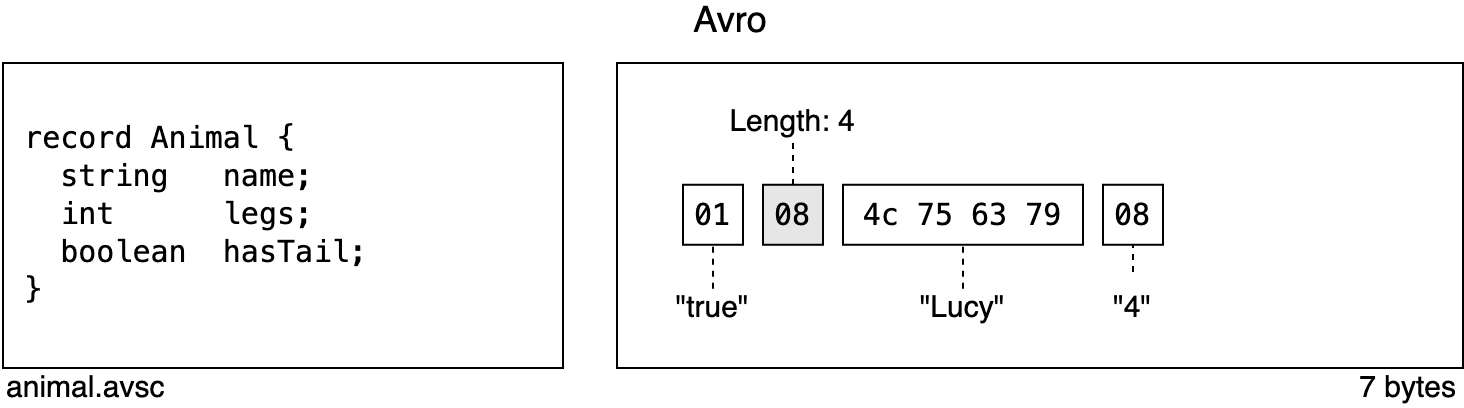
\includegraphics[height=1.5in]{avro}
    \caption{A Avro schema and its associated serialized record }
    \label{fig:avro}
\end{figure}

The deserializer knows which bytes belong to which field by comparing both the consumer and producer schemas and by matching fields by their names.

Another system that makes use of schema registries, is the Java RMI \cite{12}, a Java API that supports remote method invocation,
the object-oriented equivalent of remote procedure calls (RPC), with support for direct
transfer of serialized Java classes and distributed garbage-collection.

The Java RMI makes use of a schema registry for allowing clients to get a reference (a stub) to a remote object.
In general, an RMI registry is used only to locate the first remote object a client needs to use.
Then, typically, that first object would in turn provide application-specific support for finding references to other objects.

\paragraph{}

Our approach will need the use of a service registry, which will enhance the capabilities of a schema registry by storing not just schemas but also service-to-service dependencies.

\section{Service Evolution Approaches} % (fold)
\label{sec:service_evolution_approaches}

Due to various factors services can not keep their stability
permanently, evolution occurs throughout their entire life cycle.

Controlling and supporting the evolution of services is a significant technological research endeavor.
The paper \cite{17} proposes five standards for evaluating existing methods for evolving Web services;
these standards, and some methods are also applicable in a micro-service setting, as microservices can be viewed as web services:

\paragraph{Granularity of evolution}
Granularity refers to the unit on which the evolution is based.
Coarse-grained evolution strategies support the evolution of general interface properties,
whereas fine-grained evolution strategies support the evolution individual basic properties, such as the type of parameter in a method.

\paragraph{Terminal of evolution}
The term refers to whether the end result of a changed service affects the producer, the consumer, or both.

\paragraph{Type of evolution}
Evolutionary methods can be divided into two broad categories: semantic and architectural.
Architectural methods typically evolve changes to the composition of components, whereas semantic methods are primarily based on the semantic extension of contracts.

\paragraph{Scalability}
This standard assesses an evolutionary method's applicability and generality in different contexts.

\paragraph{Maintainability}
This standard assesses the difficulty of maintaining system's that employ the relevant evolutionary method.

\paragraph{}

The conventional approach for evolving microservices is to keep various versions of a service implementation available with a hand-off period,
and to explicitly redirect requests to the supported version.
This approach has been proven to be pragmatic, but exceedingly expensive,
because it necessitates high maintainability and partitions available resources among continually shifting subsets of consumers.
Bellow we present more effective service evolution approaches.

\subsection{Schema Resolution Rules} % (fold)
\label{sec:schema_resolution_rules}

Frameworks such as WDSL, Avro, Protocol Buffers and Thrift support schema evolution via resolution rules and declarative semantics,
where the old version of the software can deal with the new version of the service’s syntax; however, their schema evolution support is limited \cite{11}:
\begin{itemize}
    \item Only the addition, removal and renaming of fields is allowed.
    \item To ensure backwards compatibility, added fields must be optional.
    \item The only fields that can be removed to maintain forward compatibility are optional fields.
    \item To provide both forward and backward compatibility, removed and added fields must be optional.
\end{itemize}
Backward compatibility refers to a consumer using schema X to process data produced by schema X-1,
whereas forward compatibility refers to data produced by schema X being read by consumers using schema X-1.

\paragraph{}

The need for optional fields in the above cases is due to a lack of information on the consumer, typically this information is supplied with the use of default values.
In order to support required fields with backwards-forwards compatibility, the system should enforce required fields when the consumer and producer agree on the schema,
and only use default values when the consumer and producer disagree on the schema.

These limitations are problematic because, in order to enforce required fields in former case,
validation logic would need to be written repeatedly by programmers (in the same layer as the business logic).
This validation should be in a layer above because, the scale of the validation logic is proportional to the complexity of messages being validated;
for messages with more properties, particularly those with nested objects, the validation footprint can rise dramatically in terms of both line-count and logical complexity.

\paragraph{}

The aforementioned frameworks include built-in support for event-driven and RPC communication methods,
however, if a RESTful communication approach is adopted, these frameworks will be unable to manage changes in the signature of endpoints
(eg. changing the method of REST endpoint's from GET to POST); only changes in record schemas will be managed in this case.
To decrease the complexity of the evolution adaptation process, we believe it is necessary to handle both the evolution of records schemas, and the evolution of API signatures in a single integrated approach.

\subsection{Chain of adapters} % (fold)
\label{sec:chain_of_adapters}

The chain of adapters is a design strategy for providing a web service in the face of independently developed unsupervised clients while preserving strict backwards compatibility.
This approach decomposes long update/rollback transactions into smaller, independent transactions.

This technique is discussed in depth in the work \cite{13}. The key concepts of the approach are presented below.

\paragraph{}

When a new service API is published, the old API is not decommissioned;
instead, it is made available in a different namespace.
In a RESTful system, this often entails supporting operations in different versions;
Endpoints belonging to the API in v1.0 can be made accessible via the path http://example.system/v1,
whereas endpoints belonging to the API in v2.0 are accessible via the path http://example.system/v2.

The previous API implementations are replaced by adapters that redirect all calls to the next API version implementation and also translate data structures as necessary.

\paragraph{}

Updating a service's API in this manner requires the programmer to do two additional steps:
\begin{itemize}
    \item Duplicate all modified endpoints in service contract into a different namespace.
    \item Implement an adapter that translates the endpoints in version vi->vi+1.
\end{itemize}

The same web service that supports the revised service endpoints also supports the older endpoints that require adapters.
It is not necessary to deploy the web service in several versions.

When a consumer is using version v1, and the producer is using version v4, the endpoints that provide the service in version v1 use the adapters v1->v2, v2->v3, and v3->v4 to translate the operation before forwarding it to the endpoint in the current version.
The service's backwards compatibility is ensured by the composition of adapters in a chain, as seen in figure \ref{fig:chain}.

\begin{figure}[htbp]
    \centering
    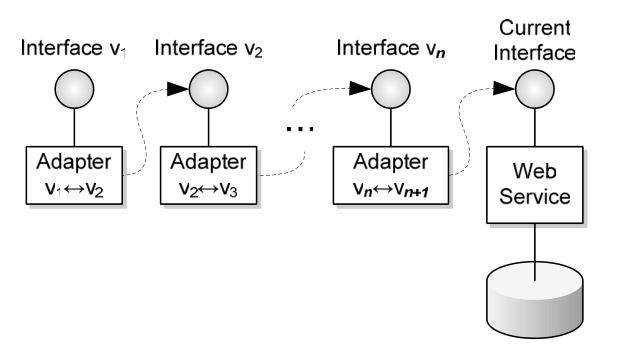
\includegraphics[height=1.5in]{chain}
    \caption{Chain of Adapters structure
    after n versions have been published }
    \label{fig:chain}
\end{figure}

\paragraph{}

The method used in this technique may be used in our solution as well.
The availability of our system can be increased by employing this method as a
placeholder adaption mechanism for when the adapter proxy is being built and initialized for earlier contract versions.

\subsection{Proxy Adapter} % (fold)
\label{sec:proxy_adapter}

This method will be explored and evaluated in our solution, the papers [] also investigates this approach.

\paragraph{}

In this strategy the knowledge of a microservice’s
interfaces is used to create a lightweight proxy capable of dynamically adapting the messages exchanged between services to match them with the static service code.

\paragraph{}

The proxy creation mechanism makes use of the available meta-information
to automatically update the proxy components as needed, adhering to a one-to-one protocol between producer and consumer services.

The proxy can be installed on either consumers or producers;
however, it is usually preferable to install the proxy on consumer services to avoid centralizing the load of message adaptation in a single point.
When the service is also consumed by externally developed clients,
it is usually beneficial to install the proxy in producers, since it is difficult to install the adapter in uncontrolled clients.

\paragraph{}

Services are initially deployed without a proxy, proxies are generated on demand using a lazy instantiation method, that creates them when the first communication between corresponding services occurs.

In essence, every communication contains information about the agreed-upon version, the handshake protocol uses this information to determine if a proxy update is required or not.
The lazy instantiation method improves the maintainability of the system by
simplifying deployment operations.

\paragraph{}

Under this approach, changes to type definitions in a producer module do not have immediate impact on the entire system by requiring global downtime.
For instance, if a consumer and producer service agree on a type definition for an given endpoint,
their existing service implementations will continue to function correctly even if that type definition evolves.

\section{Service Integration Adapters} % (fold)
\label{sec:service_integration_adapters}

There has been substantial investigation on the adaptability of services in the context of service-oriented architectures.
Although SOA \cite{7} and Microservices \cite{14} are similar in that they both use a separation approach based on services,
these two designs differ in several important ways, most notably in that microservices are loosely coupled whereas SOA services are tightly tied due to common data storage between services.
As a result, adaptability in SOA is focused on service integration and replaceability rather than evolution.

\paragraph{}

In the setting of SOA, adapters are used to wrap the various services which are in general heterogeneous,
(communicate with different protocols and support different data formats) so that they can appear as homogeneous and therefore easier to be integrated.

These adapters presume that data adaptation has already been established by developers at an upper layer,
their primary concern is merging services with different communication protocols and mismatches between operations that have the
same functionality but differ in operation name, number, order or type of operation input/output parameters.

\paragraph{}

The paper \cite{15} presents a taxonomy of all conceivable mismatches as well as remedies to each type in the context of SOA.
Some of the defined mismatches remain important in the context of microservice evolution:

\paragraph{Message Split Mismatch}
This type of differences occurs when the protocol P requires a single message to achieve certain functionality,
while in protocol PR the same behavior is achieved by receiving several messages.

\paragraph{Message Merge Mismatch}
This type of differences occurs when protocol P needs to receive several messages for achieving certain
functionality while protocol PR requires one message to achieve the same functionality.

\paragraph{Differences at the Operation Level}
This type of mismatch occurs when the operation O of S imposes constraints on input parameters,
which are less restrictive than those of OR input parameters in SR (e.g., differences in value ranges).

\paragraph{}

The two first types of mismatches can be handled in the context of microservice evolution without the use of adaptors.
Essentially, the old endpoints are kept operational but marked as deprecated until there are no more consumers using them, and the new endpoints are provided in parallel.

The latter form of mismatch has an impact on microservice evolution only if service contracts allow refined types.
In other words, when constraints in input parameter are validated in a layer above the application layer.
If validation is conducted in a lower layer, the mismatch can be easily resolved by modifying the application's implementation while keeping the service contract untouched.

\section{Deployment Strategies} % (fold)
\label{sec:deployment_strategies}

Deployment strategies are techniques that aim to provide means to upgrade a service,
while discontinuing the previous implementation without incurring downtime.

These strategies will be beneficial in the context of our solution since all service updates will evolve the immediate termination of the prior implementation,
as it is no longer required to keep several versions available to offer backwards compatibility in service contracts.
The service registry will aid in the application of these strategies, since it is responsible for managing service deployments and un-deployments.

\paragraph{}

A blue-green deployment approach is the most often used deployment strategy.
The new version (the blue version) is made available for testing and review, while users continue to use the stable version (the green version).
Users are moved to the blue version after the version passes all compliance checks.

\paragraph{}

A common alternative strategy is to have two A/B versions active at the same time, with some users using one and others using the other.
This can be used to test user interface changes and other features and gather feedback from users.
It can also be used to test proper operation in a production setting where problems affect only a few users.

\paragraph{}

A canary deployment tests the new version, but if a problem is identified, it rapidly reverts to the previous version.
This can be performed in either of the above approaches.

\paragraph{}

A rolling deployment is an alternative strategy that gradually replaces instances of an service previous version with instances of the new version.
Before scaling down the old components, a rolling deployment typically waits for new pods to become ready via a readiness check.
If a significant problem arises, the rolling deployment can be halted.

\paragraph{}

Our solution will use the rolling deployment strategy because it provides the best availability guarantees
and is natively supported by Kubernetes, the microservice orchestration tool that has been adopted.

\section{API Management Tools} % (fold)
\label{sec:api_management_tools}

API management is the process of overseeing API functions like API creation, description, testing, analysis, publication, securing, and monitoring.
All of these API management requirements can only be met with the assistance of tools, this is where API management tools enter the picture.

\paragraph{}

Microsoft Azure's API Management platform (AAMP) is a tool that provides some of the above functionalities in a manner that is similar to that of our solution.
In this platform, programmers are allowed to manually define transformations that should be performed on all responses from a microservice [].
The primary distinction is that Azure API Management transformations are intended to be specified by the programmer in policy statements,
whereas our transformations can be applied automatically without the intervention of developers.

The main use case of these transformations in AAMP is the integration of legacy backends by modernizing their APIs and making them accessible from cloud services, without the risk of migration.

\paragraph{}

In AAMP all requests from client applications are routed through the API gateway, which then forwards them to the appropriate backend services.
The API gateway, like our adapter proxy, acts as a facade to the backend services,
allowing API providers to abstract API implementations and evolve backend architecture without impacting API consumers.
The AAMP's responsibilities and functionalities include:

\begin{itemize}
    \item Accepting API calls and routing them to configured backends;
    \item Verifying API keys, JWT tokens, certificates, and other credentials;
    \item Enforcing usage quotas and rate limits;
    \item Transforming requests and responses as specified in policy statements;
    \item Caching responses to improve response latency and minimize the load on backend services;
    \item Emitting traces for monitoring, reporting, and troubleshooting;
    \item Collecting API usage metrics
\end{itemize}


We aim to include some of the aforementioned features in our service registry implementation, particularly the collection of usage metrics.
